

\documentclass[12pt]{article}
\usepackage[T1]{fontenc}
\usepackage[utf8]{inputenc}
\usepackage{amsmath}
\usepackage{microtype}
\usepackage{listings}
\setlength{\parindent}{0pt}
\usepackage{fancyvrb}
\usepackage{enumerate}
\usepackage{array}
\usepackage[breaklinks=true,linktocpage,hidelinks]{hyperref}
\usepackage[letterpaper]{geometry}
\usepackage{url}
\usepackage{graphicx}
\usepackage{fullpage}
\usepackage{caption}
\captionsetup{labelfont={bf,small,sf}, textfont={small, sf}}
\usepackage[sc]{mathpazo}

\usepackage{pgfplots}
\usepackage{pgfplotstable}
\usepackage{tikz}

\usepackage{fancyhdr}
\usepackage{fancybox}
\usepackage{multicol}
\usepackage{xcolor}
\usepackage{adjustbox}
\usepackage{wrapfig}



\pgfplotsset{compat=newest}
\usetikzlibrary{shapes,backgrounds,arrows}
\usepgfplotslibrary{external} 

\definecolor{brewcol1}{RGB}{166,206,227}
\definecolor{brewcol2}{RGB}{31,120,180}
\definecolor{brewcol3}{RGB}{178,223,138}
\definecolor{brewcol4}{RGB}{51,160,44}
\definecolor{brewcol5}{RGB}{251,154,153}
\definecolor{brewcol6}{RGB}{227,26,28}
\definecolor{brewcol7}{RGB}{237,179,1}
\definecolor{brewcol8}{RGB}{202,178,214}
\definecolor{brewcol9}{RGB}{206,27,1}

\definecolor{brewforest1}{RGB}{65,171,93}
\definecolor{brewforest2}{RGB}{161,217,155}
\definecolor{brewforest3}{RGB}{49,163,84}

\geometry{hmargin=1.87cm, vmargin=1.87cm}
\bibliographystyle{siam}

\DeclareTextFontCommand{\helvetica}{\fontfamily{phv}\selectfont\small}


\begin{document}

\clearpage\thispagestyle{empty}
\begin{center}
\textbf{Difficult transition for sugar maple in Boreal forest under climate change? \\
Impact of alternative stable states on Sugar maple migration.}
\vskip 2em
Research proposal
\vskip 1em
Master in Wildlife management
\vfill
By
\vfill
Steve Vissault 
\vfill 
For
\vfill
\textbf{Richard Cloutier}, Pr.\\
Director of the program committee
\vskip 2em
\textbf{Dominique Arsenault}, Pr.\\
President of the jury
\vskip 2em
\textbf{Matt Talluto}, PhD\\
Research Co-director
\vskip 2em
\textbf{Dominique Gravel}, Pr.\\
Research Director
\vfill
\vfill
Université du Québec à Rimouski\\
\today

\end{center}

\newpage
\setcounter{page}{1}

\section{Introduction}

\textbf{Context.}  The boreal region is warming twice as fast as the global
average and will inevitably alter species composition in boreal forest
\cite{Scheffer2012,Hughes2000}.  Sugar maple is one of those species expected
to migrate northward towards it's nordic temperate forest limits
\cite{McKENNEY2007,Goldblum2005}. Predict shifts in the repartition of sugar
maple under climate change is an important challenge whereas this species is
highly coveted by hardwood and maple syrup producers, two main economic
sectors in Quebec. Indeed, Sugar maple is a widespread and abundant tree in
north- eastern North America and one of the most representative species of
northern temperate forests \cite{Graignic2013,Messaoud2007,Kellman2004}. This
northward migration will result in increasing the surface of the ecotone
between the boreal and temperate forest of Quebec. Nevertheless, the expansion
of species distribution occuring in Nordic temperate forest could be difficult
and explain by the fact than microclimatic conditions found in boreal forests
are different from those present in temperate forest. Colder temperatures from
shading and excess soil moisture due to snow melt cause litter to be more
acidic and fibrous during the spring. Therefore, even if the regional climate
conditions are favorable \cite{Kellman2004}, the microbiota conditions found
in the boreal forest could affect the establishment of sugar maple
\cite{Kellman2004,Moore2008,DeFrenne2013,Barras1998}. In this case, the sugar
maple could be unable to migrate in boreal forests as a result of negative
soil feedback. This phenomen could increase the tension between the boreal
forest and the nordic temperate forest and generating abrupt changes in the
community composition (\textbf{$H_0$}). \textbf{Objectives.} This project aim to develop
a state and transition model (STM) between the boreal and temperate nordic
forest in order to investigate shifts in the distribution of sugar maple into
the boreal-temperate forest dynamical system.To assess this main objective, we
will (1) generate a transitional model between the temperate and the boreal
forest; (2) investigate the spatial structure of the transitonnal zone; and
finaly (3) run simulations based on different climate change scenarios. To
realized those objectives, we will use the alternative stable states theory as
a framework. In order to define the context of this study, the first section
is a review subdivided into two paragraphs. The first part will present the
theorical context on the alternative stable states and abrupt changes in
ecosystems functionning. Second part of this section will focus on the Sugar
maple and his community and thus explain why is alternative stable states a
relevant framework to study the dynamic of the boreal-temperate forests
ecotone.  The second section of this document will describe the model and the
methodology employed to assess the objectives. To conclude, the last part will
present the general timeline associated to this project. 

\section{Review} \textbf{Theorical framework.}  Many ecotone studies and
modeling efforts on transition between forest to none-forest ecosystems (e. i.
Boreal - Toundra) \cite{Scheffer2012,Scheffer2001,Hirota2011} but little
attention has been given to evaluate the transitional dynamics of forest-
forest ecotone \cite{Goldblum2010,Graignic2013}. At large scale, transition
between  the temperate nordic and the boreal forests can be approach as a
dynamic system where each forest biomes is a state. The presence of different
states at a location or a time depends on environmental conditions (e. i.
Soil, temperature) encountered by the system. When small environnemental
fluctuations occurs, mostly dynamical system can respond almost linearly with
no particular threshold to observe drastic changes in state of the ecosystem (
Figure \ref{fig1} .A) \cite{Scheffer2001,Scheffer2009}. Thus, increase the
soil moisture might cause favorable conditions to a new species, but doesn't
affect the functionning of the ecosystem. In this case, only one equilibrium
can be observed given a specific environnemental condition
\cite{Scheffer2001,Scheffer2009,scheffer2009critical}. Another kind of system
response occurs more frequently in nature.  Natural systems are rather
insensitive over certain ranges of environnementals conditions while
responding strongly when a treshold is reached by the system (Figure
\ref{fig1} .B) \cite{scheffer2009critical}. Tree mortality can increase
sharply when a specific toxicant level is added in the environment.
\cite{scheffer2009critical}. In this case, the respond curve of the natural
systeme is lightly folded but small forcing can conduct at large changements
as the entire transformation in species community composition. In an other
hand, respond curve can be folded backwards and the same threshold can conduct
the system into catastrophic changes (Figure \ref{fig1} .C). In this
situation, the system present alternative stable states who mean the
possibility to get two different contrasted stable states for a certain range
of environnemental conditions, called hysteresis zone (Figure \ref{fig1} .C).
\textbf{More description} In the Boreal-temperate nordic forest ecotone, there
is no distinct boundary instead, a broad transition zone exists composed of
mixed stands of coniferous and deciduous species \cite{Goldblum2010}. Instead,
a macromosaic landscape can be observed with pure stands of deciduous trees on
favorable sites and pure coniferous stands on less favorable sites found on
poor soils \cite{Goldblum2010}. Assuming this fact, the alternative stable
states is a relevant framework to study this ecotone dynamic therefore the
soil seems to have a negative feedback on the temperate forest establishment
and need to be investigate has a main attractor in alternative stable states
\cite{Kellman2004,Moore2008,DeFrenne2013,Barras1998}. \\

\begin{figure}[t]       
	\begin{center}
		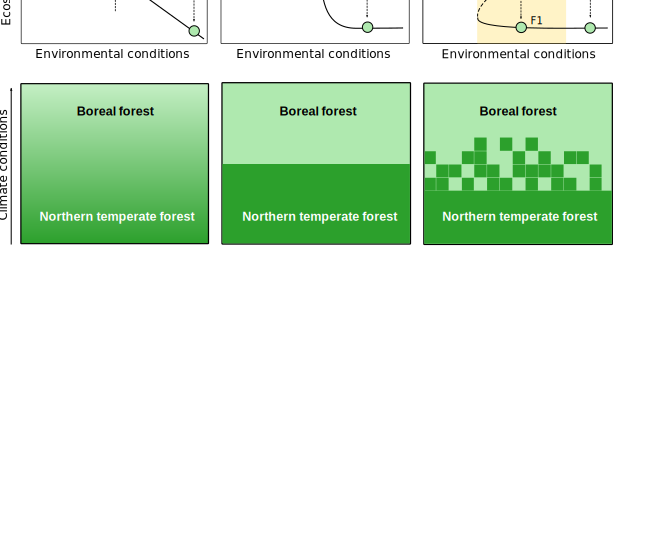
\includegraphics[width=0.8\textwidth]{fig/states.pdf}       
	\end{center}
	\caption{Schematic representation of different ways in which the equilibrium
	state of a system can vary with conditions such as temperature, precipitation
	or soil moisture. Three differents kinds of respond are presented,
	\textbf{(A)} gradual, \textbf{(B)} basic fold, \textbf{(C}) catastrophic fold.
	The first panels line is a conceptualization of a transitional landscape
	between the boreal (light green) and the nordic temperate forests (dark
	green). The second panels line presents the stable states rise by the forest
	given a specific environnemental condition. Each arrows in graphs indicate the
	point toward the system moves if it's not at the equilibrium. Every point on
	the plain line could be a stable state encounter by the boreal-temperate
	forests system, excepted for the dashed line (in yellow highlight). This zone,
	called hysteresis, are particulary unstable and little fluctuations in
	environnement conditions give rise to a contrasted state representing an
	alternative stable states.  ($F_1$ or $F_2$).}
		\label{fig1}
\end{figure}

\textbf{Natural system.} 
% L'écotone entre la forêt boréal et la forêt tempérée
% nordique. La répartition des espèces caractéristiques de ces milieux ne sui
% pas un gradient climatique mais concorde avec un gradient lié à la texture et
% à la composition du sol. Plusieurs espèces clés représentent fortement les
% communautés végatles rattachés à ces biomes. Ces espèces germent sur des
% conditions de sols contrastés contribuant à maintenir la présence


% We used maple sugar basa areal in function of black
% spruce, white spruce and balsam fir basal area to compute the relative
% abundance of sugar maple. Given the above statements, we used mainly two
% climatic variables (annual mean temperature and annual precipitation) to
% identify the alternative stable states present in the boreal-temperate
% ecotone. The relationship was performed on climatic variables and sugar maple
% relative abundance using kernel density plot function. We obtained the
% probability of observed a sample plot as function of sugar maple relative
% abundance and mean annual temperature (Figure \ref{fig1}). In both case,
% alternative stable states are presents whereas the function graphed has a
% bimodal distribution. At low precipitation or temperature conditions, the
% probability of observing a parcel sampled without sugar maple is higher than
% intermediate climatic conditions where the multimodal distribution appear. The
% density function suggest the presence of alternative stabe states  in response
% of intermediate climatic conditions: one state wherein sugar maple dominates
% and an another in which sugar maple is absent. \\

\section{Methods}   

\begin{wrapfigure}{l}{0.45\textwidth}
		
	\begin{figure}[!ht]
\begin{center}
	
				\tikzstyle{noeud}=[circle,
				                  thick,
				                  minimum size = 1.5cm,
				                  inner sep =5pt,
				                  draw=brewforest3,
				                  fill=brewforest1]
				\tikzstyle{noeud2}=[circle,
				                  thick,
				                  minimum size = 1.5cm,
				                  inner sep =5pt,
				                  draw=brewforest3,
				                  fill=brewforest2]
				\tikzstyle{noeud3}=[circle,
				                  thick,
				                  minimum size = 1.5cm,
				                  inner sep =5pt,
				                  draw=brewforest3,
				                  fill=brewforest3]
	
				\begin{tikzpicture}[->,>=stealth',auto,scale=0.8]
				      \node [circle,noeud2] (M) at (0,0) {\textbf{M}};
				      \node [circle,noeud2]  (C) at (-5,5) {\textbf{C}};
				      \node [circle,noeud2] (D) at (5,5) {\textbf{D}};
				      \node [circle,noeud2] (T) at (0,10) {\textbf{T}};
	
						\draw[thick,-latex] (M) to[bend right=10] node[above,sloped] {$S_C$} (C);
						\draw[thick,-latex] (C) to[bend right=10] node[below,sloped] {$\beta_d \cdot (C+M)$} (M);
	
						\draw[thick,-latex] (D) to[bend right=10] node[above,sloped] {$\beta_c \cdot (D+M)$} (M);
						\draw[thick,-latex] (M) to[bend right=10] node[below,sloped] {$S_D$} (D);
	
						\draw[thick,-latex] (D) to[bend right=10] node[above,sloped] {$e$} (T);
						\draw[thick,-latex] (T) to[bend right=10] node[below,sloped] {$P_D$} (D);
	
						\draw[thick,-latex] (T) to[bend right=10] node[above,sloped] {$P_C$} (C);
						\draw[thick,-latex] (C) to[bend right=10] node[below,sloped] {$e$} (T);
	
						\draw[thick,-latex,transform canvas={xshift=0.8ex}] (T) to node[above,sloped,rotate=90,transform canvas={xshift=5ex}] {$P_D \cdot P_C$} (M);
						\draw[thick,-latex,transform canvas={xshift=-0.8ex}] (M) to node[above,sloped,rotate=-90,transform canvas={xshift=-3ex}] {$e$} (T);
				\end{tikzpicture}
	
			\caption{Conceptual transition model between forest stands deciduous ($D$), mixte ($M$) and coniferious ($C$). $E$ corresponds to a transitionnal state where a perturbation are occurred with a frequence of $e$. Parameters $\beta$ and $S$ are referred as the colonisation and the succession rates respectively. We defined the recovery rates ($P_C$ et $P_D$) as $P_C = \alpha_C \cdot (M+C) \cdot [1- \alpha_D \cdot (D +M)]$ and $P_D = \alpha_D \cdot (D+M) \cdot [1- \alpha_C \cdot (C +M)]$, to finaly get this equation $P_M = P_C \cdot P_D$. The parameter $\alpha$ mean the recovery rate after a patch has been disturbe.}

	\end{center}	
	\label{Model}
\end{figure}
		\caption{Conceptual transition model between forest stands deciduous ($D$), mixte ($M$) and coniferous ($C$). $T$ corresponds to a transitionnal state where a perturbation are occurred with a frequence of $e$. Parameters $\beta$ and $S$ are referred as the colonisation and the succession rates respectively. We defined the recovery rates ($\phi_C$ et $\phi_D$) as $\phi_C = \alpha_C \cdot (M+C) \cdot [1- \alpha_D \cdot (D +M)]$ and $\phi_D = \alpha_D \cdot (D+M) \cdot [1- \alpha_C \cdot (C +M)]$, to finaly get this equation $\phi_M = \phi_C \cdot \phi_D$. The parameter $\alpha$ mean the recovery rate after a patch has been disturbe.}
		\label{Model}
\end{wrapfigure}

\textbf{Models.} This state and transition model will be based on three
differents states characterizing the boreal and nothern temperate forests
landscape: \textbf{(D)} Deciduous; \textbf{(C)} Coniferous;  \textbf{(M)}
Mixed stand (Figure \ref{Model}) and finaly Transition patch \textbf{(T)}.The
general overview allow to say that all states can be convert to another state
excepted the direct transition between a deciduous  and coniferous stands who
don't appear frequently in natural system considering the contrasted
environnement (i.e. soil, moisture).  Simulations of this model aims to assess
the transition rate between each state in the overall landscape and identify
if deciduous and coniferious patches are present as alternative stable states.
To embed the climat component, each model parameters will be calibrate as a
function of probability based on climatic conditions. Climat is a main driver
in the distribution of those biomes, but their dynamics are strongly related
to their own disturbance regimes (i. e. Fire in boreal forest, frost in
temperate forest) \cite{Goldblum2010}.  Thus the disturbance component has
been integrated within the model accross the transitional patch (T) (Figure
\ref{Model}). When a coniferous patch $C$ has been disturbed with a rate $e$,
this can be recovered to another state following $\phi_C$. This term is taking
in account a specific patch recovery rate ($\alpha_{C}$), the availability of
coniferous species ($M+C$) and the proportion of paths unconverted into a
deciduous state ($1- \alpha_D \cdot (D +M)$). In making the assumption that
perturbation rate is similar between states, dynamic of a patch $T$ can be
formally describe by this differential equations: $\frac{\delta T}{\delta t} =
e \cdot (C+M+D) -  T \cdot (\phi_D + \phi_C + \phi_M)$. If this patch $C$ is
undisturbed, deciduous species $(D+M)$ can spread over the patch with a
colonisation rate $\beta_d$  giving a new mixed patch. This mixed stand $M$
might be transform later into a coniferous stand with a sucessional rate
$S_C$.  We can also summarize the coniferous dynamic by this differential
equation: $\frac{\delta C}{\delta t} = \phi_C \cdot T + S_C \cdot M - \alpha_D \cdot
(D+M)\cdot C - e \cdot C$. At this stage of this project, this model is
spatially implicit and assume that all space is occupied by one state, so that
the proportions of land cover occupied by all types of patch sum to 1.  \\

\textbf{Paramerization.} The parameterization of this model will be conducted
on the QUICC-FOR database containing large permanent sample plots surveys.
Those data are provided by several forest offices and cover multiple canadian
provinces ($\pm16 000$ plots) and states (\textbf{Ask at Miranda} plots).
These inventories started since the 1970s and include all stems measurements
and forest stand informations relative to a specific plot location and year.
In a first time, the basal area will be compute to provide a measure of
relative growth by species present in the plots. \\

\textbf{Simulation.} This model will be incorporated in a spatially explicit cellular automaton or lattice in
order to evaluate the velocity of the transition into differents patches and differents
climate change scenario.

% - Temps discrets
% - Cellulaire automate\\

\textbf{Validation.} 
% - Matrice de confusion sur la classification des patchs (M,D,C,T)
% - Matrice de confusion (TSS) et AUC sur un jeux de données indépendants 
% - Spatialement explicit à l'aide de l'automate cellulaire.


\newpage
\bibliography{/home/steve/Dropbox/Bibtex/Devis}
\end{document}

%%%%%%%%%%%%%%%%%%%%%%%%%%%%%%%%%%%%%%%% 
%%% Extra

%We will assume that all space is occupied by one state, so that the proportions of land cover occupied by all types of patch sum to 1.

%\frac{\delta C}{\delta t} = \alpha_C \cdot (C+M) \cdot (1-\alpha_D \cdot (D+M)) \cdot (1-C-D-M) + S_C \cdot M - \%beta_D \cdot (D+M) \cdot C - e \cdot C%
%\frac{\delta D}{\delta t} = \alpha_D \cdot (D+M) \cdot (1-\alpha_C \cdot (C+M)) \cdot (1-C-D-M) + S_D \cdot M - %\%beta_C \cdot (C+M) \cdot D - e \cdot D
%\frac{\delta M}{\delta t} = \alpha_C \cdot (C+M) \cdot \alpha_D \cdot (D+M) \cdot (1-C-D-M) + \beta_C \cdot (C+M) + \beta_D \cdot (D+M) - S_C \cdot M - S_D \cdot M - e \cdot M

% \begin{figure}[!ht]
% 	\centering
% 	\begin{minipage}{0.45\linewidth}
% 		
	\begin{figure}[!ht]
\begin{center}
	
				\tikzstyle{noeud}=[circle,
				                  thick,
				                  minimum size = 1.5cm,
				                  inner sep =5pt,
				                  draw=brewforest3,
				                  fill=brewforest1]
				\tikzstyle{noeud2}=[circle,
				                  thick,
				                  minimum size = 1.5cm,
				                  inner sep =5pt,
				                  draw=brewforest3,
				                  fill=brewforest2]
				\tikzstyle{noeud3}=[circle,
				                  thick,
				                  minimum size = 1.5cm,
				                  inner sep =5pt,
				                  draw=brewforest3,
				                  fill=brewforest3]
	
				\begin{tikzpicture}[->,>=stealth',auto,scale=0.8]
				      \node [circle,noeud2] (M) at (0,0) {\textbf{M}};
				      \node [circle,noeud2]  (C) at (-5,5) {\textbf{C}};
				      \node [circle,noeud2] (D) at (5,5) {\textbf{D}};
				      \node [circle,noeud2] (T) at (0,10) {\textbf{T}};
	
						\draw[thick,-latex] (M) to[bend right=10] node[above,sloped] {$S_C$} (C);
						\draw[thick,-latex] (C) to[bend right=10] node[below,sloped] {$\beta_d \cdot (C+M)$} (M);
	
						\draw[thick,-latex] (D) to[bend right=10] node[above,sloped] {$\beta_c \cdot (D+M)$} (M);
						\draw[thick,-latex] (M) to[bend right=10] node[below,sloped] {$S_D$} (D);
	
						\draw[thick,-latex] (D) to[bend right=10] node[above,sloped] {$e$} (T);
						\draw[thick,-latex] (T) to[bend right=10] node[below,sloped] {$P_D$} (D);
	
						\draw[thick,-latex] (T) to[bend right=10] node[above,sloped] {$P_C$} (C);
						\draw[thick,-latex] (C) to[bend right=10] node[below,sloped] {$e$} (T);
	
						\draw[thick,-latex,transform canvas={xshift=0.8ex}] (T) to node[above,sloped,rotate=90,transform canvas={xshift=5ex}] {$P_D \cdot P_C$} (M);
						\draw[thick,-latex,transform canvas={xshift=-0.8ex}] (M) to node[above,sloped,rotate=-90,transform canvas={xshift=-3ex}] {$e$} (T);
				\end{tikzpicture}
	
			\caption{Conceptual transition model between forest stands deciduous ($D$), mixte ($M$) and coniferious ($C$). $E$ corresponds to a transitionnal state where a perturbation are occurred with a frequence of $e$. Parameters $\beta$ and $S$ are referred as the colonisation and the succession rates respectively. We defined the recovery rates ($P_C$ et $P_D$) as $P_C = \alpha_C \cdot (M+C) \cdot [1- \alpha_D \cdot (D +M)]$ and $P_D = \alpha_D \cdot (D+M) \cdot [1- \alpha_C \cdot (C +M)]$, to finaly get this equation $P_M = P_C \cdot P_D$. The parameter $\alpha$ mean the recovery rate after a patch has been disturbe.}

	\end{center}	
	\label{Model}
\end{figure}
% 	\end{minipage}
% 	\begin{minipage}[t]{1\linewidth}
% \small{\begin{equation}
% 	 	\frac{\delta T}{\delta t} = e \cdot (C+M+D) -  T \cdot (\phi_D + \phi_C + \phi_M \\
% \end{equation}
% \begin{equation}
% 		\frac{\delta M}{\delta t} = \phi_M\cdot T +  \beta_C \cdot (C+M)\cdot D + \beta_D\cdot (D+M)\cdot C - S_C\cdot M -S_D\cdot M - e\cdot M \\
% \end{equation}
% \begin{equation}
% 		\frac{\delta C}{\delta t} = \phi_C \cdot T + S_C\cdot M - D\cdot (D+M)\cdot C - e \cdot C \\
% \end{equation}
% \begin{equation}
% 		\frac{\delta D}{\delta t} = \phi_D \cdot T + S_D \cdot M - \beta_C \cdot (C+M) \cdot D - e \cdot D
% \end{equation}}
% 	\end{minipage}
